\documentclass[options]{beamer}

\usetheme{Madrid}

\usepackage[utf8]{inputenc}
\usepackage{amssymb, amsmath, amsfonts, amsthm}
\usepackage{mathrsfs}
\usepackage{verbatim}
\usepackage{hyperref}

\usepackage{minted}
\usepackage{tikz}
\usetikzlibrary{shapes, arrows}


\title{Fast* Implementations of Finite Fields \\ and Elliptic Curves in Lean 4}
\author{Matej Penciak}
\institute{Lurk Lab}
\date{March 23, 2023 \\ Slides available at: \\ \url{https://github.com/mpenciak/LLL2023}}
\titlegraphic{
\includegraphics[width = .14\textwidth]{img/lurk_lab_logo.png}}

\begin{document}

\frame{\titlepage}

\begin{frame}
    \frametitle{Outline}
    \begin{enumerate}
        \item Motivation: What we're building at Lurk Lab
        \item A bit about zero knowledge cryptography
        \item Optimizing FF arithmetic
        \begin{itemize}
            \item Addition chains for fast exponentiation
            \item Batched inversion
            \item Montgomery form
        \end{itemize}
        \item Optimizing elliptic Curve arithmetic
        \begin{itemize}
            \item Choice of coordinates
            \item Efficient endomorphisms
            \item Multi-scalar multiplication
        \end{itemize}
        \item Brief demo!
        \item Lessons learned and future outlook
    \end{enumerate}
\end{frame}

\begin{frame}[fragile]
    \frametitle{Motivation}
    {\bf Who am I?} Software engineer and aspiring cryptographer at Lurk Lab (Formerly Yatima).

    \pause
    \vspace{5pt}

    {\bf What is Lurk Lab?} We're building the Lurk programming language, and an ecosystem of tools around it.
    Examples: The Yatima compiler and content addresser, a Lean typechecker, and the cryptography to generate ``Lurk proofs''

    \pause
    \vspace{5pt}

    {\bf What is Lurk?} Lurk is a turing complete programming language in the style of Lisp which generates zero knowledge proofs of execution.

    \pause
    \vspace{5pt}

    If I run a Lurk program \verb+f+, I can prove things like:
    \begin{itemize}
        \item I have run the computation of \verb+f+ applied to \verb+u+ and gotten \verb+v+
        \item I know an input \verb+u+ to \verb+f+ such that \verb+f(u) = v+ without revealing \verb+u+
        \item I can commit ahead of time to a program \verb+f+ and run it on any inputs $\{$\verb+u+$\}$ you provide with proofs of execution.
    \end{itemize}

\end{frame}

\begin{frame}[fragile]
    \frametitle{A little about zero knowledge proofs}

    Two components to a zero knowledge proof system:
    \begin{itemize}
        \item An interactive proof scheme (the ``information-theoretic'' component)
        \item A commitment scheme (the ``cryptographic'' component)
    \end{itemize}

    \vspace{7pt}
    \pause

    An {\bf IP scheme} is a protocol between two parties \verb+P+ (prover) and \verb+V+ (verifier)
    where (the potentially untrustworthy) \verb+P+ can provide a convincing argument to \verb+V+ that they know some fact/have performed some computation.
    
    \vspace{7pt}
    \pause

    A {\bf commitment scheme} is an interactive protocol for one party to commit to some data (a vector, polynomial, etc...) without revealing its value. The commitment can be opened later, and it should be computationally infeasible for the committer to change their committed value

\end{frame}

\begin{frame}[fragile]
    \frametitle{An example IP}

    \verb+P+ and \verb+V+ agree to two graphs $G_1$ and $G_2$, and \verb+P+ wants to prove to \verb+V+ that they know an isomorphism $\phi : G_1 \to G_2$ without revealing the isomorphism.

    \pause

    \begin{enumerate}
        \item \verb+P+ chooses a random permutation $\sigma$ of $G_1$, and sends $H = \sigma(G_1)$ to  \verb+V+
        \item \verb+V+ chooses randomly between $\{1, 2\}$ and sends the choice $i$ to \verb+P+
        \item \verb+P+ responds with an isomorphism $\phi_i : G_i \to H$
        \item \verb+V+ checks that in fact $\phi_i(G_i) \cong H$
        \item Repeat until \verb+V+ is sufficiently convinced
    \end{enumerate}

    \pause 
    This protocol is {\bf complete}, {\bf knowledge sound}, and {\bf zero knowledge}

    \vspace{5pt}
    \pause

    It is not: {\bf non-interactive}, or {\bf succinct}

    The goal is to build {\bf Z}ero {\bf K}nowledge {\bf S}uccinct {\bf Ar}guments of {\bf K}nowledge (ZK SNARKs) in Lean.
\end{frame}

\begin{frame}
    \frametitle{The basic building blocks for cryptography}

    %Add some cryptography to the IPs:

    Work over finite fields, and encode our computations in so-called ``arithmetic circuits''.

    The level of security necessary is measured in the number of ``bits'' of security. To prevent a dishonest prover from forging a fraudulent proof, a good estimate is $\approx 128$ bits of security.
    
    \vspace{6pt}
    \pause

    {\bf Example 1}: The fastest (publicly) known factorization/discrete logarithm algorithm is the general number field sieve method with complexity
    $$\mathrm{exp}\left(\left(\sqrt[3]{\frac{64}{9}} + o(1)\right)(log n)^{\frac{1}{3}} (\log \log n)^{\frac{2}{3}}\right)$$

    To achieve $\approx 128$ bits of security we need to work over finite fields of size $\approx 2^{2048}$
\end{frame}

\begin{frame}
    \frametitle{Elliptic curve cryptography}

    
    {\bf Example 2}: Let $E$ be an elliptic curve with a cyclic subgroup of points of size $N$.
    
    The best (publicly) known discrete logarithm algorithm (given $P = a \cdot G$, find $a \in \mathbb{N}$) is the Pollard-$\rho$ method which has complexity $O(\sqrt{N})$.

    To achieve $\approx 128$ bits of security we only need a curve with $\approx 2^{256}$ number of points.

    \vspace{6pt}
    \pause
    
    Hasse's bound, makes it ``easy'' to find elliptic curves with enough points -- if $E$ is an elliptic curve defined over a finite field with $p$ elements, then the number of points $N$ is bounded by:

    $$\left| N - (p + 1)\right| \leq 2 \sqrt{p}$$

    When we discuss curves, we will see some magical curves with extra nice properties

\end{frame}
\begin{frame}[fragile]
    \frametitle{Big numbers in Lean}

    Most computers don't natively support arithmetic for numbers larger than $2^{64} - 1$, stored in the Lean datatype \verb+UInt64+.

    Lean 4's \verb+Nat+ and \verb+Int+ types are built on multiprecision arithmetic libraries written in C(++), and linked in via the \verb+@[extern "..."]+ attribute
    \begin{minted}{Lean}
    @[extern "lean_nat_add"]
    protected def Nat.add : (@& Nat) → (@& Nat) → Nat
        | a, Nat.zero   => a
        | a, Nat.succ b => Nat.succ (Nat.add a b)
    \end{minted}

    \vspace{6pt}
    \pause
    
    which calls the C function defined in \verb+lean.h+

    \begin{minted}{c}
    static inline lean_obj_res 
        lean_nat_add(b_lean_obj_arg a1, b_lean_obj_arg a2) {
         . . .
    }
    \end{minted}
\end{frame}

\begin{frame}[fragile]
    \frametitle{Multiprecision arithmetic libraries}

    Lean uses the {\bf G}NU {\bf M}ulti{\bf P}recision library on Linux based systems. Mac and Windows get a home-brewed version written in the Lean 4 C++ runtime code.

    \vspace{6pt}
    \pause

    Both implementations represent \verb+Nat+s as arrays of \verb+UInt64+s, and define arithmetic in base $2^{64}$. If $n$ is the number of ``limbs'' (\verb+uint64_t+s in C) then the efficiency of some of the most commonly employed algorithms are:

    \begin{enumerate}
        \item Schoolbook multiplication: $O(n^2)$

        \item Karatsuba multiplication: $O(n^{1.58})$
              
        \item Strassen FFT algorithm: $O(n \log n \log \log n)$
    \end{enumerate}

    \vspace{6pt}
    \pause

    We tried using fixed precision arithmetic based off Lean's \verb+ByteArray+ type instead of \verb+Nat+.

    This turned out to be $\approx 100 \times$ slower than \verb+Nat+, so we quickly dropped that plan.

\end{frame}

\begin{frame}[fragile]
    \frametitle{A comment on benchmarking and testing}

    Testing and benchmarking is important for non-formalized systems.

    For testing we have built a testing framework called \verb+LSpec+ which is expressive and easy to use.

    \pause
    \vspace{6pt}

    \begin{minted}{Lean}
    #lspec check "add_comm"
        (forall n m : Nat, n + m = m + n)
    #lspec check "not true" 
        (forall n m : Nat, n^2 + m^2 >= n^3 + m)
    \end{minted}

    \vspace{6pt}

    \begin{verbatim}
    ? add_comm
    x not true
    ===================
    Found problems!
    n := 2
    m := 0
    issue: 8 <= 4 does not hold
    (1 shrinks)
    \end{verbatim}
\end{frame}

\begin{frame}[fragile]
    \frametitle{A comment on benchmarking and testing}

    For benchmarking we have a rudimentary suite of tools for running benchmarks:

    \begin{minted}{lean}
    import YatimaStdLib.Benchmark
    import YatimaStdLib.AddChain

    open Benchmark

    def f1 : Nat → Nat := (37 ^ .)
    def f2 : Nat → Nat := Exp.fastExp 37
    def addChainBench : Comparison f1 f2 where
        inputs := #[10000000, 15000000,  ...]

    def main (args : List String) : IO UInt32 := 
        benchMain args addChainBench.benchmark
    \end{minted}

\end{frame}

\begin{frame}[fragile]
    \frametitle{Benchmarking continued...}

    This can be run as \verb+Benchmarks-AddChain --num 50 --log out.bench+
    and times the benchmarks and writes to the file:

    \begin{verbatim}
    10000000: f:213993503 vs g:236587657
    15000000: f:315046597 vs g:335218176
    20000000: f:457342988 vs g:537591730
    25000000: f:598272104 vs g:681122849
    30000000: f:670924537 vs g:743308727
    35000000: f:786821581 vs g:940891049
    40000000: f:950924114 vs g:1103080520
    45000000: f:1108323608 vs g:1213150412
    50000000: f:1242277288 vs g:1288141664
    \end{verbatim}

\end{frame}

\begin{frame}[fragile]
    \frametitle{Back to fields}

    The arithmetic typeclasses we have (so far):

    \begin{itemize}
        \item \verb+Ring+: Basic arithmetic: $+$, $*$, and so on
        \item \verb+Field+: Ring together with inversion
        \item \verb+PrimeField+: Arithmetic, plus pre-computations and methods to improve efficiency
        \item \verb+NewField+: Automatically generated instance of a \verb+PrimeField+ with special methods related to Montgomery form
        \item \verb+GaloisField+: Fields obtained as extension fields of a base field
    \end{itemize}

    \vspace{6pt}
    \pause
    No \verb+Prop+ valued fields! Nothing is formalized (yet).

\end{frame}

\begin{frame}
    \frametitle{Field typeclasses}

    \begin{tikzpicture}[node distance=3cm]
        \node (ring) [draw, rectangle] {Ring};
        \node (field) [draw, rectangle, right of=ring] {Field};
        \node (primefield) [draw, rectangle, above right of=field] {PrimeField};
        \node (newfield) [draw, rectangle, right of=primefield] {NewField};
        \node (galoisfield) [draw, rectangle, below right of=field] {GaloisField};
        
        \draw [->] (ring) -- (field);
        \draw [->] (field) -- (primefield);
        \draw [->] (field) -- (galoisfield);
        \draw [->] (primefield) -- (newfield);
    \end{tikzpicture}

    (thanks ChatGPT)

\end{frame}

\begin{frame}[fragile]
    \frametitle{Example classes}

\begin{minted}{lean}
class Ring (R : Type _) extends Add R, Mul R, Sub R, 
        HPow R Nat R, BEq R, Coe Nat R where
    zero : R
    one : R
\end{minted}

\begin{minted}{lean}
class PrimeField (K : Type _) extends Field K where
    char : Nat -- characteristic
    sqrt : K → Option K -- Fast `sqrt` implementation
    content : Nat -- char.log2
    twoAdicity : Nat x Nat -- `(s, r)` where `p-1 = 2^s * r'
    legAC : Array ChainStep  -- Pre-computed AddChains to
    frobAC : Array ChainStep -- calculate .^p and .^(p-1)/2
    fromNat : Nat → K -- to and from `Nat`' methods
    natRepr : K → Nat
    batchedExp : K → Array Nat → Array K
    batchedInv : Array K → Array K
\end{minted}

\end{frame}

\begin{frame}[fragile]
    \frametitle{AddChains, batched arithmetic, and Montgomery form}

    {\bf AddChains}: Exponentiation is a commonly used operation, but can be very slow.

    Naive implementation: $a ^ N = a \cdot a^ {N -1}$ is $O(N)$ (too slow)

    \pause
    \vspace{6pt}

    Square and multiply method requires $\approx \frac{3}{2} \log N$ operations

    ($\log N$ squarings plus the Hamming weight of $N$'s binary expansion)
    ({\bf WARNING}: susceptible to side channel attacks)

    \pause
    \vspace{6pt}

    For commonly used exponents ($p$ and $\frac{p-1}{2}$): pre-compute a minimal length``addition chain'':
    $[n_1, n_2, n_3, ..., n_r = N]$ where each $n_i = n_k + n_l$ for $k, l < i$. 

    \pause
    \vspace{6pt}

    {\bf Example}: Calculating the Frobenius modulo the prime:
    \begin{small} \verb+0x40000000000000000000000000000000224698fc094cf91b992d30ed00000001+ \end{small}
    $381$ field ops using square and multiply, and $337$ field ops using a minimal addition chain.
\end{frame}

\begin{frame}
    \frametitle{Batched inversion}

    {\bf Batched inversion}:

    Inversion is another costly operation (inversion in $\mathbb{Z}/p\mathbb{Z}$ is $O(\log p)$ using the extended Euclidean algorithm)

    To invert $[n_1, n_2, n_3, \ldots, n_r]$, calculate $N_j = \prod_i^j n_i$ for $j = 1, \ldots, r$ caching the results. Invert $N_r$. Recover all of the $n_i^{-1}$ by multiplying with the cached results. 

    \vspace{6pt}
    \pause

    {\bf Example:} Inverting the set $[2, 3, 5]$.
    
    \begin{enumerate}
        \item Calculate $N_1 = 2$, $N_2 = 6$, $N_3 = 30$. 
    
        \item Invert $N_3$ : $N_3^{-1} = 30^{-1}$, let $t = N_3^{-1}$
        
        \item Multiply $t \cdot N_2 = 30^{-1} \cdot 6 = 5^{-1}$, and $t = t \cdot n_3 = 6^{-1}$
        
        \item Proceed as before: $t \cdot N_1 = 6^{-1} \cdot 2 = 3^{-1}$, and $t = t \cdot n_2 = 2^{-1}$
    \end{enumerate}

    This method replaces $r$ field inversions with $1$ field inversion and $O(3r)$ field multiplications. 
\end{frame}

\begin{frame}[fragile]
    \frametitle{Montgomery form}

    {\bf Problem}: How should we calculate $n \cdot m$ in $\mathbb{F}_p$ when we use \verb+Nat+ representatives?

    Naive algorithm: Calculate $a \cdot b \mod p$, but this requires division by $p$ for every multiplication. 

    \pause
    \vspace{6pt}

    {\bf Intuition behind the solution}: Replace reduction modulo $p$ with reduction modulo $R$ for some other $R$.

    Let $R > p$ be a number co-prime to $p$ for which division and reduction modulo $R$ is efficient. 

    In practice: Choose $R$ to be a power of 2 greater than $p$.

    Represent $n \in \mathbb{Z} / p \mathbb{Z}$ in "Montgomery form" $[n]_w = n \cdot R \mod p$.

    Montgomery reduction is an efficient algorithm that calculates $n R^{-1} \mod p$ using only arithmetic modulo $R$.

    \vspace{6pt}
    \pause

    Addition: $[n]_w + [m]_w = (n + m) \cdot R \mod p = [n + m]_w$

    Multiplication: $[n]_w \cdot [m]_w = (n \cdot m) R^2 \mod p = [n \cdot m]_w R \mod p$ \\
    $\longrightarrow$ Montgomery reduce $[n \cdot m]_w$
\end{frame}

\begin{frame}[fragile]
    \frametitle{NewField implementation}

    We implemented a \verb+macro_rule+ that expands the following declaration

    \begin{minted}{lean}
    new_field TestField with
        prime: 2011
        generator: 7
        root_of_unity: 2010 -- optional
    \end{minted}

    into a type \verb+TestField+ with pre-computations and arithmetic, instances, and methods implemented. 

    \vspace{6pt}
    \pause

    Not advised to be used yet: Missing some key GMP methods to make Montgomery reduction more efficient
    (\verb+mpz_tdiv_r_2exp+).

    \vspace{6pt}

    Part of Montgomery reduction of $a\cdot R \in \mathbb N$ involves working modulo $R$, which is not more efficient in Lean at this time.

\end{frame}
\begin{frame}[fragile]
    \frametitle{Elliptic Curves}

    Immediate goals are to work with curves defined over fields of large characteristic, so short Weierstrass form is fine:

    \begin{minted}{lean}
/--
Curves with Weierstrass form satisfying the equation 
`y² = x³ + a x + b` for a prime field `F` such that 
`char K > 3`
-/
structure Curve (F : Type _) [Field F] where
    a : F
    b : F
    \end{minted}

\end{frame}

\begin{frame}[fragile]
    \frametitle{Arithmetic on curves}

    Arithmetic is more interesting:
    
    \begin{minted}{lean}
class CurveGroup {F : outParam $ Type _} [Field F] 
        (K : Type _) (C : outParam $ Curve F)  where 
    zero : K
    inv : K → K
    add : K → K → K
    double : K → K
    \end{minted}
    
    \vspace{6pt}
    \pause

    Separating the curve from its arithmetic is important to allow for different coordinate systems on the same curve.

    \vspace{6pt}
    \pause
    
    Projective coordinates avoid field inversions!

    Affine coordinates are more compact on disk!

    More exotic coordinate systems have other benefits.

\end{frame}

\begin{frame}
    \frametitle{Coordinate breakdown}
    \begin{figure}[h]
    \caption{Chart taken from \emph{Handbook of Elliptic and Hyperelliptic Curve Cryptography}}
    \centering
    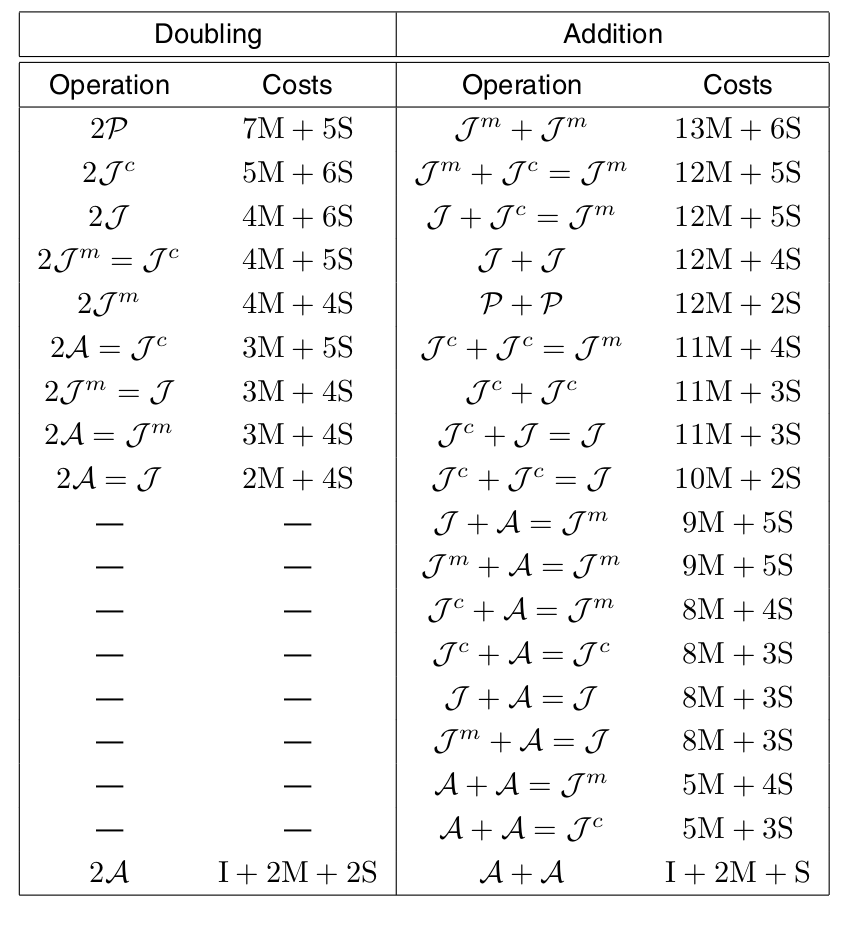
\includegraphics[height = .75\textheight]{img/coordinate_breakdown.png}
    \end{figure}
\end{frame}

\begin{frame}
    \frametitle{Naiive vs. Actual implementation}
    \begin{center}
    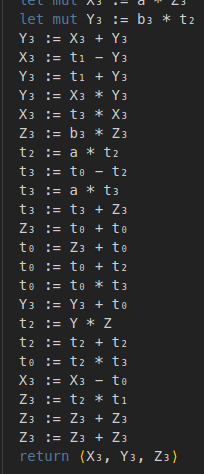
\includegraphics[height = .70\textheight]{img/screenshot.png}
    \end{center}

    Reason: Ensure Lean is evaluating the arithmetic expressions to minimize finite field operations.
\end{frame}

\begin{frame}[fragile]
    \frametitle{Scalar multiplication and GLV optimization}

    Given $n \in \mathbb{N}$ and $P \in C$, want to calculate $n \cdot P$.

    \vspace{6pt}
    \pause

    If $C$ has prime order $q$, and an efficiently computable endomorphism $\Phi : C \to C$ then
    $\Phi(P) = \Lambda \cdot P$ for some $\Lambda \in \mathbb{N}$.

    Given $n \in \mathbb N$, calculate find $n_1$ and $n_2$ of size $O(\sqrt n)$ such that
    
    $$
    n = n_1 + \Lambda n_2 \mod q
    $$

    \vspace{6pt}
    \pause

    Use this to compute 

    $$n \cdot P = (n_1 + \Lambda n_2) \cdot P = n_1 \cdot P + n_2 \cdot \Phi(P)$$

    \vspace{6pt}
    \pause

    If the curve $C$ is defined as $y^2 = x^3 + b$ then $\Phi:(x : y : z) \mapsto (\zeta x : y : z)$ for $\zeta \in \mu_3$ works.

    \pause
    \vspace{6pt}

    This optimization was subject to the patent \verb+US7995752B2+
    \emph{Method for accelerating cryptographic operations on elliptic curves}
    which expired in 2020

\end{frame}

\begin{frame}[fragile]
    \frametitle{Some very magical curves}
    
    The curve $y^2 = x^3 + 5$ defined over over $\mathbb{F}_p$ and $\mathbb{F}_q$ with primes \\ $p = $ 
    \begin{small}\verb+0x40000000000000000000000000000000224698fc094cf91b992d30ed00000001+\end{small}
    (Pallas)
    and \\ $q = $
    \begin{small}\verb+0x40000000000000000000000000000000224698fc0994a8dd8c46eb2100000001+\end{small}
    (Vesta) 

    \vspace{6pt}
    \pause

    Nice properties of the Pasta curves:
    \begin{enumerate}
        \item $\#(E_{\text{Pallas}}) = q$ and $\#(E_{\text{Vesta}}) = p$
        \item Efficiently computable endomorphism for the GLV optimization.
        \item Large 2-adicity ($p-1$ is divisible by $2^{32}$)
        \item Both primes are of the form $2^{255} + \epsilon$ which helps with reduction in $\mathbb F_p$
        \item Both have low-degree isogenies with non-zero $j$-invariant (helps with generating random points on the curves).
    \end{enumerate}

\end{frame}

\begin{frame}
    \frametitle{Multiscalar Multiplication}

    The multi-exponentiation problem: Given a set of list of integers $[n_1, n_2, \ldots, n_r]$ and a list of group elements $[g_1, g_2, \ldots, g_r]$ calculate $\prod_i^r g_i^{n_i}$.

    Multi-exponentiation in the context of elliptic curve groups asks to calculate $\sum_i^r n_i \cdot G_i$ for points $G_i \in C$. 

    \vspace{10pt}
    \pause

    Used throughout ECC (signature schemes, commitment schemes, zero knowledge proof schemes). 

    In some protocols, $\approx 80\%$ of time in generating zero knowledge proofs is spent calculating multiscalar multiplications.

    \vspace{6pt}

    Typical $r$ varies greatly by application, but can get up to sizes like $2^{28}$.
\end{frame}

\begin{frame}
    \frametitle{Pippenger's algorithm}

    Pippenger's algorithm is one of the most efficient optimizations over the naive implementation.
    
    Suppose the elliptic curve group order is approximately $b$ bits large. Pick a ``window size'' $c$ ($\log r$ turns out to be optimal) so that $b \approx k \cdot c$. 
    \begin{enumerate}
        \item  Decompose each $n_i = n_{i, 0} + n_{i, 1} \cdot 2^c + n_{i, 2} \cdot 2^{2c} + \ldots + n_{i, k} \cdot 2^{k c}$
        \item Split up the large $b$-bit MSM into $k$ separate $c$-bit MSMs:
        $$
        T_i = \sum_j^r n_{j, i} G_i
        $$
        \item Solve each $c$-bit MSM and recombine as $M = \sum_i^k 2^i \cdot T_i$. 
        
        (perfect opportunity for parallelization)
    \end{enumerate}

\end{frame}

\begin{frame}
    \frametitle{Pippenger algorithm}

    We have reduced to the case of an MSM $T = \sum_i^r n_i \cdot G_i$ where each $n_i$ is at most $c$-bits.

    \begin{enumerate}
    \item Keep track of $2^c - 1$ ``buckets'', and place each $G_i$ into the $n_i$ bucket.
    \item Sum up all the sets of points to get $2^c$ bucket sums $S_j$ for $j = 0, \ldots, 2^c - 1$
    \item $T = S_{2^c -1} + (S_{2^c -1} + S_{2^c -2}) + \ldots + (S_{2^c -1} + S_{2^c -2} + \ldots + S_0)$
    \end{enumerate}

    The Lean implementation provides an $\approx 10 \times$ speedup over the naive implementation.

    Further optimizations exist when each $G_i$ is a fixed shape relative to a generator for the elliptic curve group.

    A common case is when $G_i = \tau^i \cdot G$ for $i = 0, \ldots, r$ and $G$ is a fixed generator for the elliptic curve group.
\end{frame}

\begin{frame}
    \frametitle{A small Demo!}

    All of the above can be found:

    \vspace{30pt}

    \url{https://github.com/yatima-inc/FFaCiL.lean}
    \vspace{20pt}

    \url{https://github.com/yatima-inc/yatimastdlib.lean}


\end{frame}
\begin{frame}
    \frametitle{Lessons learned}

    \begin{enumerate}
        \item Squeezing performance out of Lean can sometimes feel like squeezing water from a stone.
        \item Lean 4 does not have ``zero cost abstractions''. 
        \item Lean 4 is early in its life, so there are few guides written down for writing efficient code.
        \item There are some significant performance pits to fall in if one isn't careful with the reference counting.
        \pause
        \vspace{10pt}
        \item Lean 4 is incredibly expressive, it's easy to prototype complex structures and algorithms that \emph{just work} on the first try.
        \item The resulting code is beautiful, and very easy to read.
        \item With time, more FFI work, and more effort I'm certain performance can be competitive.
    \end{enumerate}

\end{frame}

\begin{frame}[fragile]
    \frametitle{Future goals}

    \begin{enumerate}
        \item (short term) Optimize, optimize, optimize! (deeper GMP integration, more curve forms, ...).
        \item (short-medium term) Expand \verb+FFaCiL+ to include more elliptic curve cryptography (isogenies!).
        \item (short-medium term) Actually take advantage of dependent types.
        \item (medium term) Begin exploring the formalization of provable security (formalizing adversarial games, and complexity).
        \item (long term) Expand the Yatima Standard Library with more number theoretic primitives.
        \item (Long term) Begin the process of formally verifying these algorithms!
        \item (Epochs from now) Combine all of these efforts together into a \verb+cryptolib+ with formally verified cryptographic algorithms.
    \end{enumerate}

\end{frame}

\begin{frame}
    \frametitle{Thank you for your time!}
    \begin{center}
    Thanks!
    \end{center}
\end{frame}

\begin{frame}
    \frametitle{References}

    TODO

\end{frame}
\end{document}